\documentclass{article}
\usepackage[T1]{fontenc}
\usepackage{lmodern}
\usepackage{graphicx}
\usepackage{amsmath,amssymb}
\usepackage[a4paper,margin=2cm]{geometry}
\usepackage[absolute,overlay]{textpos}
\setlength{\TPHorizModule}{1mm}
\setlength{\TPVertModule}{1mm}
\usepackage[indonesian]{babel}
\usepackage{hyperref}
\setlength{\emergencystretch}{2em}
% unit: Halaman 27

\begin{document}

% === Halaman 27 (llm) ===

\vspace{225.72mm}

Satu putaran di dalam DES:

% deskripsi: Diagram alur satu putaran (round) dalam algoritma enkripsi DES, menunjukkan proses pengolahan L, R, C, dan D dengan fungsi F, XOR, S-box, dan permutasi.
% bbox normalisasi: [0.1700, 0.1800, 0.7600, 0.9400]
\begin{textblock*}{123.90mm}(35.70mm,53.46mm)
\noindent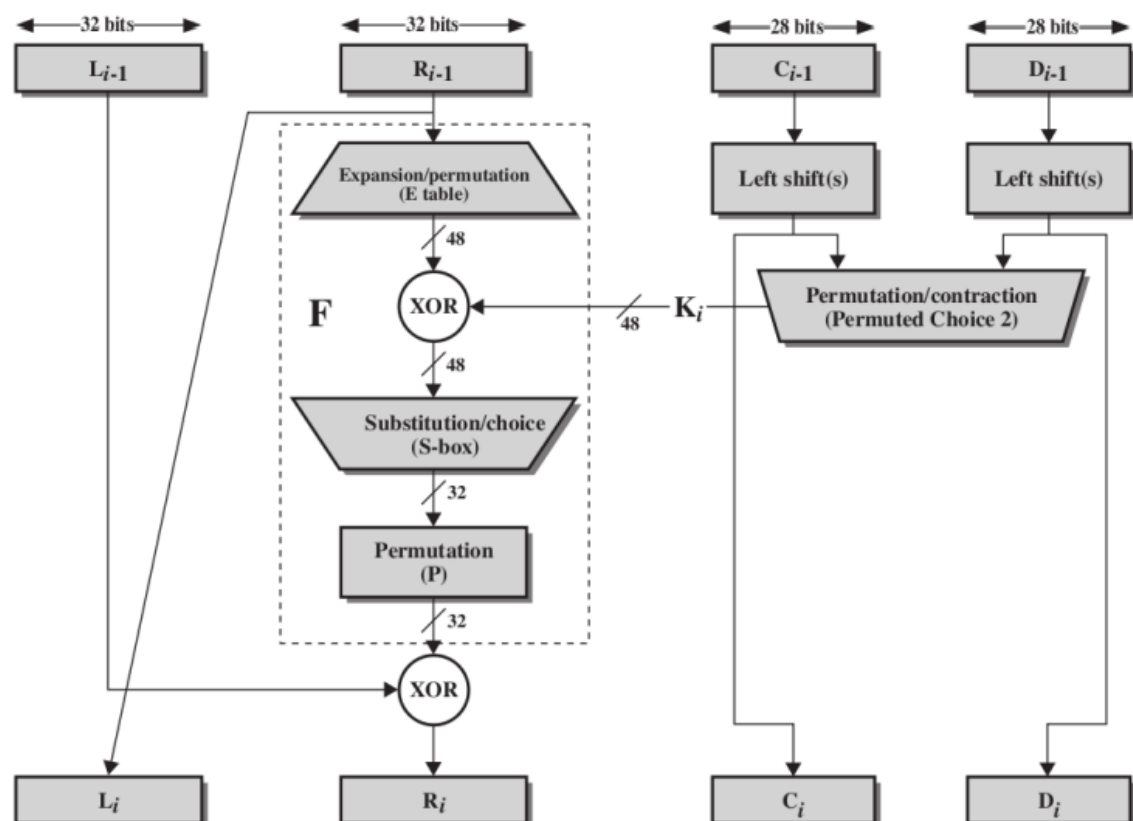
\includegraphics[width=123.90mm,height=225.72mm]{../../images/llm/page_027_img_01.png}%
\end{textblock*}

\end{document}
